\documentclass[dvipsnames,14pt,t]{beamer}
\usepackage{slides}
\usepackage{langs}
\usepackage{graph}
\usepackage{data}
\usepackage{proof}

% beamer stuff 
\renewcommand{\slidecaption}{ITP ????}
\newcommand{\bl}[1]{\textcolor{blue}{#1}}


\begin{document}
%%%%%%%%%%%%%%%%%%%%%%%%%%%%%%%%%%%%%%%%%%%%%%%%%%%%%%%%%%%%%%%%%
\begin{frame}[t]
\frametitle{%
  \begin{tabular}{@ {}c@ {}}
  \\
  \Large POSIX Lexing with Derivatives\\[-1.5mm] 
  \Large of Regular Expressions\\
  \Large (Proof Pearl)\\[-1mm] 
  \end{tabular}}\bigskip\bigskip\bigskip

  \normalsize
  \begin{center}
  \begin{tabular}{c}
  \small Fahad Ausaf\\
  \small King's College London\\
  \\
  \small joint work with Roy Dyckhoff and Christian Urban
  \end{tabular}
  \end{center}

\end{frame}
%%%%%%%%%%%%%%%%%%%%%%%%%%%%%%%%%%%%%%%%%%%%%%%%%%%%%%%%%%%%%%%%%%     

%%%%%%%%%%%%%%%%%%%%%%%%%%%%%%%%%%%%%%%%%%%%%%%%%%%%%%%%%%%%%%%%%%
\begin{frame}[c]
\frametitle{Regular Expressions}


\begin{textblock}{6}(2,5)
  \begin{tabular}{rrl@ {\hspace{13mm}}l}
  \bl{$r$} & \bl{$::=$}  & \bl{$\varnothing$}   & null\\
           & \bl{$\mid$} & \bl{$\epsilon$}      & empty string\\
           & \bl{$\mid$} & \bl{$c$}             & character\\
           & \bl{$\mid$} & \bl{$r_1 \cdot r_2$} & sequence\\
           & \bl{$\mid$} & \bl{$r_1 + r_2$}     & alternative / choice\\
           & \bl{$\mid$} & \bl{$r^*$}           & star (zero or more)\\
  \end{tabular}
  \end{textblock}
  
\end{frame}
%%%%%%%%%%%%%%%%%%%%%%%%%%%%%%%%%%%%%%%%%%%%%%%%%%%%%%%%%%%%%%%%%%   

%%%%%%%%%%%%%%%%%%%%%%%%%%%%%%%%%%%%%%%%%%%%%%%%%%%%%%%%%%%%%%%%%%
\begin{frame}[c]
\frametitle{The Derivative of a Rexp}

\large
If \bl{$r$} matches the string \bl{$c\!::\!s$}, what is a regular 
expression that matches just \bl{$s$}?\bigskip\bigskip\bigskip\bigskip

\small
\bl{$der\,c\,r$} gives the answer, Brzozowski (1964), Owens (2005)
``\ldots have been lost in the sands of time\ldots''
\end{frame}
%%%%%%%%%%%%%%%%%%%%%%%%%%%%%%%%%%%%%%%%%%%%%%%%%%%%%%%%%%%%%%%%%%   

%%%%%%%%%%%%%%%%%%%%%%%%%%%%%%%%%%%%%%%%%%%%%%%%%%%%%%%%%%%%%%%%%%
\begin{frame}[c]
\frametitle{Correctness}

It is a relative easy exercise in a theorem prover:

\begin{center}
\bl{$matches(r, s)$}  if and only if  \bl{$s \in L(r)$} 
\end{center}\bigskip

\small
where \bl{$matches(r, s) \dn nullable(ders(r, s))$}

\end{frame}
%%%%%%%%%%%%%%%%%%%%%%%%%%%%%%%%%%%%%%%%%%%%%%%%%%%%%%%%%%%%%%%%%%   

%%%%%%%%%%%%%%%%%%%%%%%%%%%%%%%%%%%%%%%%%%%%%%%%%%%%%%%%%%%%%%%%%%
\begin{frame}[c]
\frametitle{POSIX Regex Matching}

Two rules:

\begin{itemize}
\item Longest match rule (``maximal munch rule''): The 
longest initial substring matched by any regular expression 
is taken as the next token.

\begin{center}
\bl{$\texttt{\Grid{iffoo\VS bla}}$}
\end{center}\medskip

\item Rule priority:
For a particular longest initial substring, the first regular
expression that can match determines the token.

\begin{center}
\bl{$\texttt{\Grid{if\VS bla}}$}
\end{center}
\end{itemize}\bigskip\pause

\small
\hfill Kuklewicz: most POSIX matchers are buggy\\
\footnotesize
\hfill \url{http://www.haskell.org/haskellwiki/Regex_Posix}

\end{frame}
%%%%%%%%%%%%%%%%%%%%%%%%%%%%%%%%%%%%%%%%%%%%%%%%%%%%%%%%%%%%%%%%%% 

%%%%%%%%%%%%%%%%%%%%%%%%%%%%%%%%%%%%%%%%%%%%%%%%%%%%%%%%%%%%%%%%%%
\begin{frame}[c]
\frametitle{POSIX Regex Matching}

\begin{itemize}

\item Sulzmann \& Lu came up with a beautiful
idea for how to extend the simple regular expression 
matcher to POSIX matching/lexing (FLOPS 2014)\bigskip\bigskip

\begin{tabular}{@{\hspace{4cm}}c@{}}
  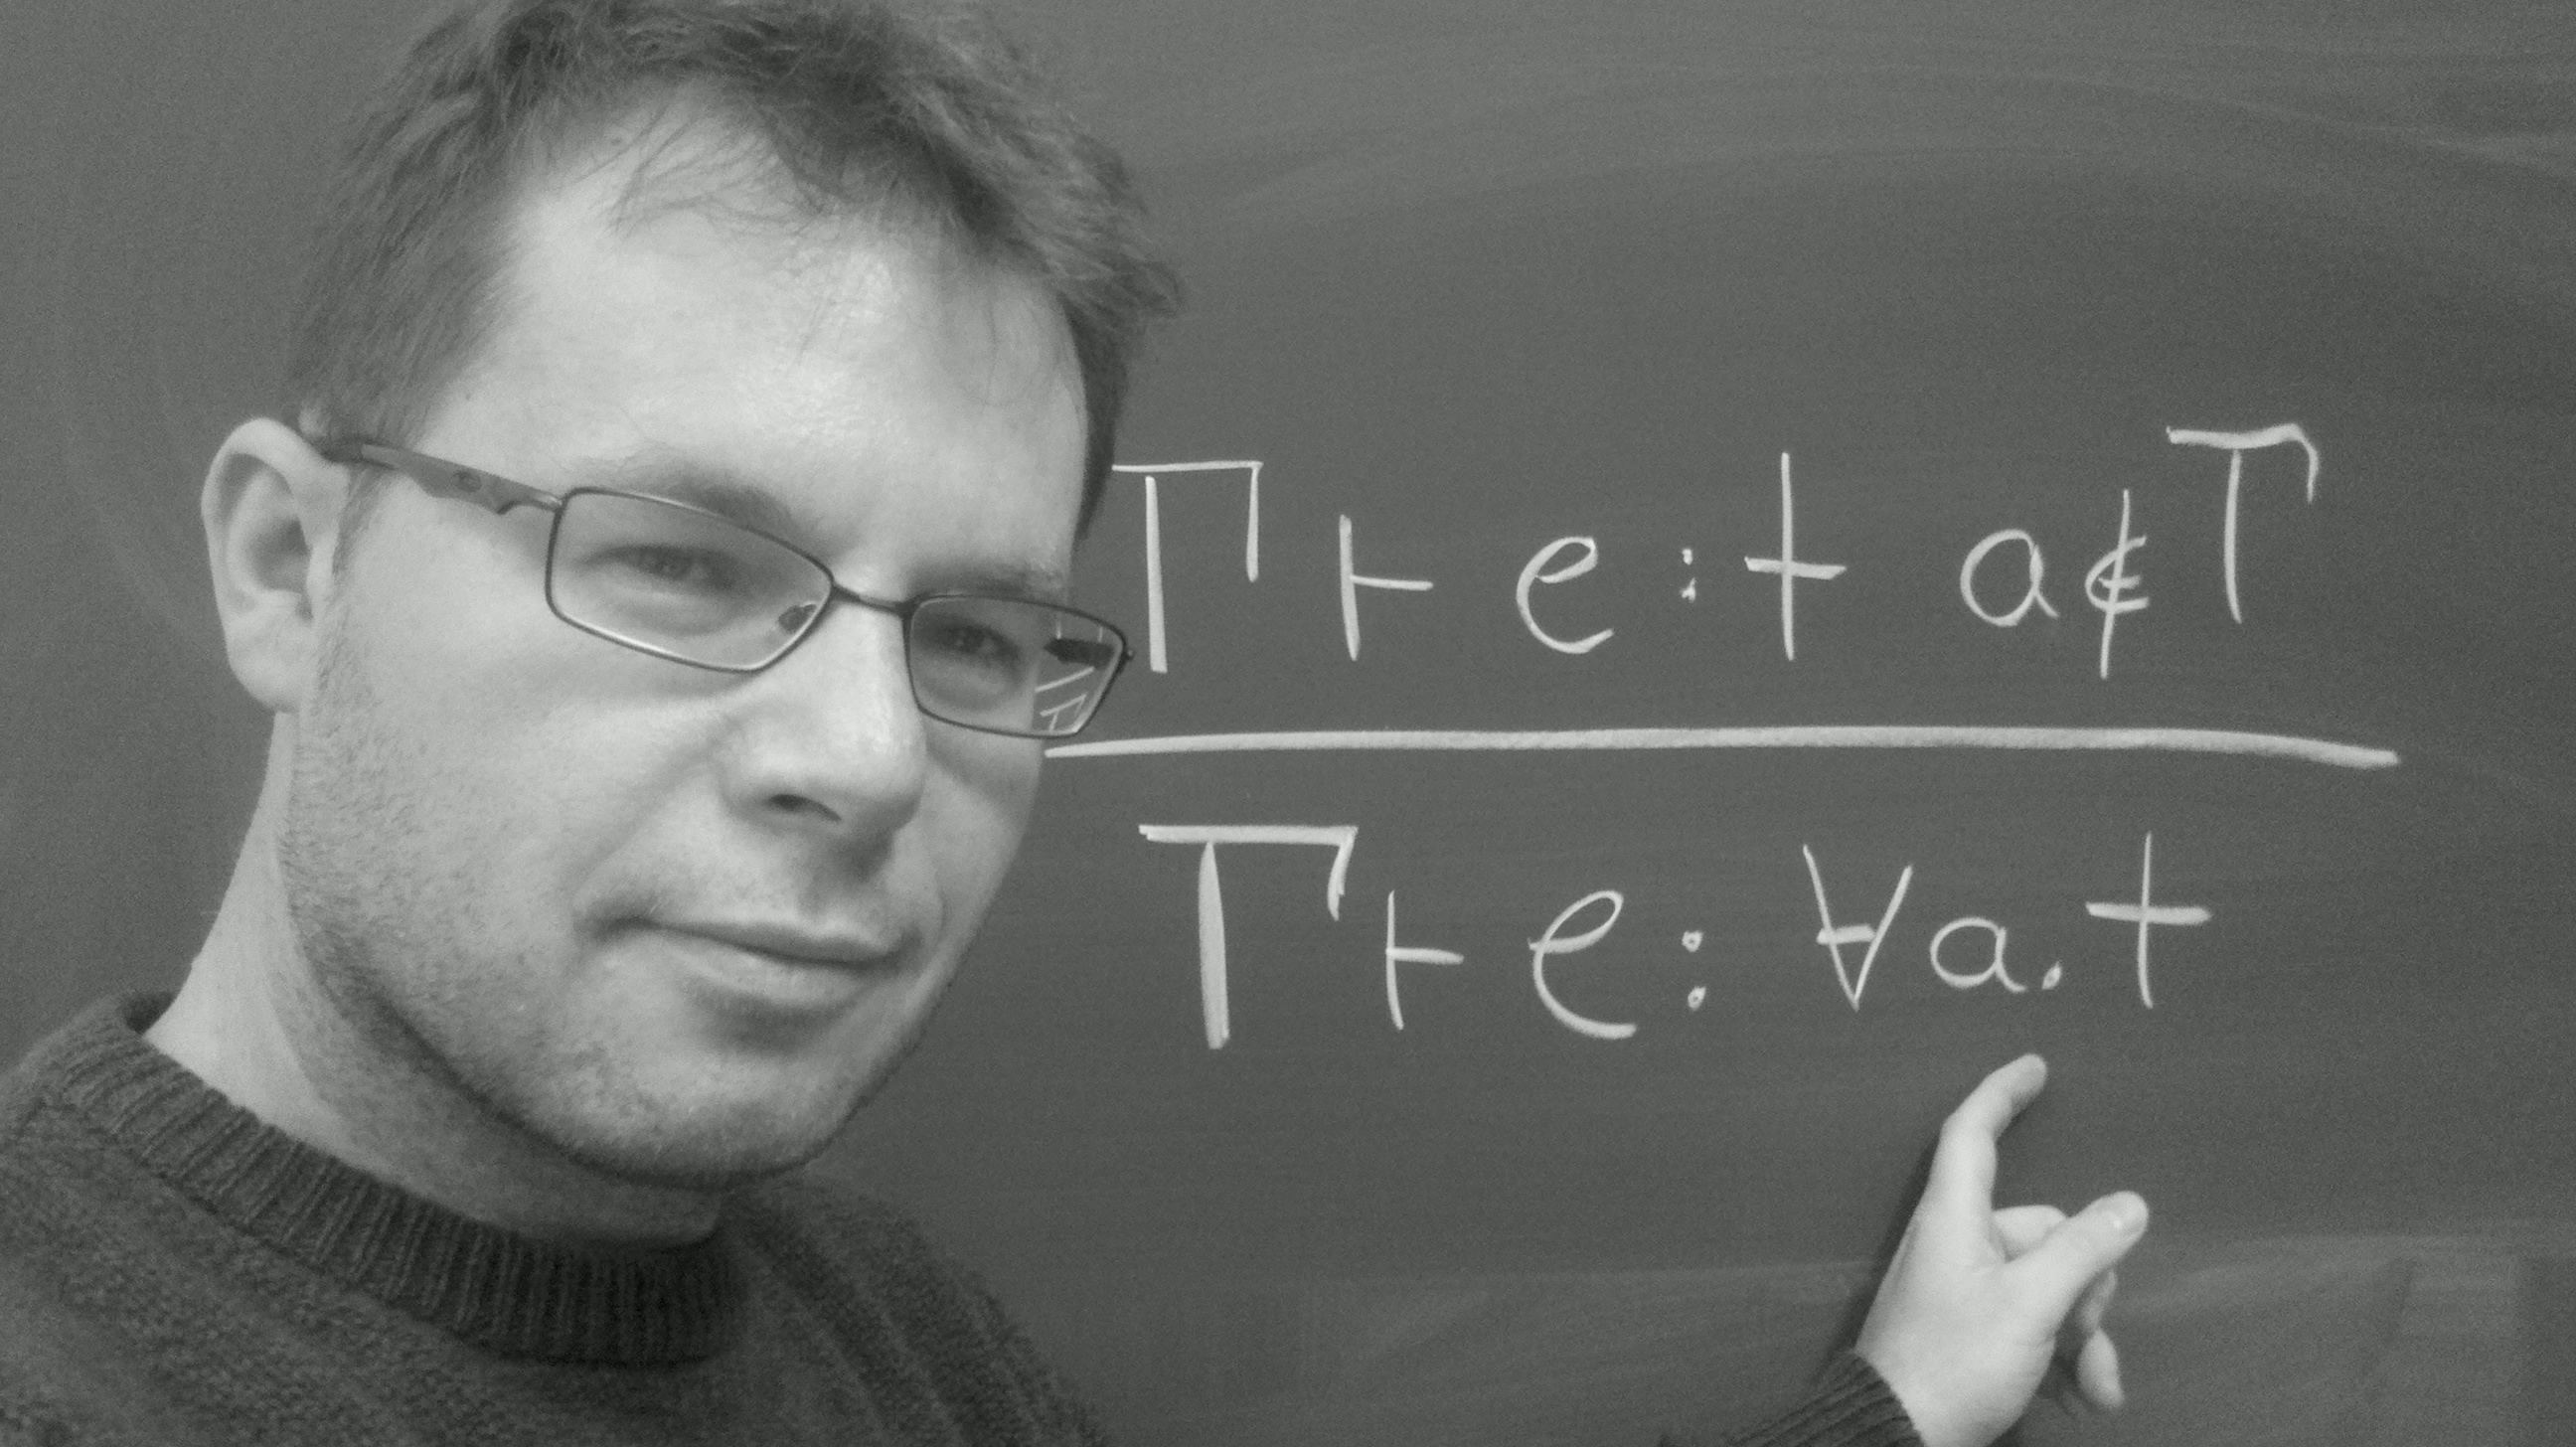
\includegraphics[scale=0.20]{pics/sulzmann.jpg}\\[-2mm]
  \hspace{0cm}\footnotesize Martin Sulzmann
\end{tabular}\bigskip\bigskip

\item the idea: define an inverse operation to the derivatives
\end{itemize}



\end{frame}
%%%%%%%%%%%%%%%%%%%%%%%%%%%%%%%%%%%%%%%%%%%%%%%%%%%%%%%%%%%%%%%%%% 


%%%%%%%%%%%%%%%%%%%%%%%%%%%%%%%%%%%%%%%%%%%%%%%%%%%%%%%%%%%%%%%%%%
\begin{frame}[c]
\frametitle{Regexes and Values}

Regular expressions and their corresponding values
(for \emph{how} a regular expression matched a string):

\begin{center}
\begin{columns}
\begin{column}{3cm}
\begin{tabular}{@{}rrl@{}}
  \bl{$r$} & \bl{$::=$}  & \bl{$\varnothing$}\\
           & \bl{$\mid$} & \bl{$\epsilon$}   \\
           & \bl{$\mid$} & \bl{$c$}          \\
           & \bl{$\mid$} & \bl{$r_1 \cdot r_2$}\\
           & \bl{$\mid$} & \bl{$r_1 + r_2$}   \\
  \\
           & \bl{$\mid$} & \bl{$r^*$}         \\
  \\
  \end{tabular}
\end{column}
\begin{column}{3cm}
\begin{tabular}{@{\hspace{-7mm}}rrl@{}}
  \bl{$v$} & \bl{$::=$}  & \\
           &             & \bl{$Empty$}   \\
           & \bl{$\mid$} & \bl{$Char(c)$}          \\
           & \bl{$\mid$} & \bl{$Seq(v_1,v_2)$}\\
           & \bl{$\mid$} & \bl{$Left(v)$}   \\
           & \bl{$\mid$} & \bl{$Right(v)$}  \\
           & \bl{$\mid$} & \bl{$[]$}      \\
           & \bl{$\mid$} & \bl{$[v_1,\ldots\,v_n]$} \\
  \end{tabular}
\end{column}
\end{columns}
\end{center}\pause

There is also a notion of a string behind a value: \bl{$|v|$}

\end{frame}
%%%%%%%%%%%%%%%%%%%%%%%%%%%%%%%%%%%%%%%%%%%%%%%%%%%%%%%%%%%%%%%%%%   


%%%%%%%%%%%%%%%%%%%%%%%%%%%%%%%%%%%%%%%%%%%%%%%%%%%%%%%%%%%%%%%%%%
\begin{frame}[c]
\frametitle{Sulzmann \& Lu Matcher}

We want to match the string \bl{$abc$} using \bl{$r_1$}:

\begin{center}
\begin{tikzpicture}[scale=2,node distance=1.3cm,every node/.style={minimum size=8mm}]
\node (r1)  {\bl{$r_1$}};
\node (r2) [right=of r1] {\bl{$r_2$}};
\draw[->,line width=1mm]  (r1) -- (r2) node[above,midway] {\bl{$der\,a$}};\pause
\node (r3) [right=of r2] {\bl{$r_3$}};
\draw[->,line width=1mm]  (r2) -- (r3) node[above,midway] {\bl{$der\,b$}};\pause
\node (r4) [right=of r3] {\bl{$r_4$}};
\draw[->,line width=1mm]  (r3) -- (r4) node[above,midway] {\bl{$der\,c$}};\pause
\draw (r4) node[anchor=west] {\;\raisebox{3mm}{\bl{$\;\;nullable?$}}};\pause
\node (v4) [below=of r4] {\bl{$v_4$}};
\draw[->,line width=1mm]  (r4) -- (v4);\pause
\node (v3) [left=of v4] {\bl{$v_3$}};
\draw[->,line width=1mm]  (v4) -- (v3) node[below,midway] {\bl{$inj\,c$}};\pause
\node (v2) [left=of v3] {\bl{$v_2$}};
\draw[->,line width=1mm]  (v3) -- (v2) node[below,midway] {\bl{$inj\,b$}};\pause
\node (v1) [left=of v2] {\bl{$v_1$}};
\draw[->,line width=1mm]  (v2) -- (v1) node[below,midway] {\bl{$inj\,a$}};\pause
\draw[->,line width=0.5mm]  (r3) -- (v3);
\draw[->,line width=0.5mm]  (r2) -- (v2);
\draw[->,line width=0.5mm]  (r1) -- (v1);
\draw (r4) node[anchor=north west] {\;\raisebox{-8mm}{\bl{$mkeps$}}};
\end{tikzpicture}
\end{center}

\only<10>{
The original ideas of Sulzmann and Lu are the \bl{\textit{mkeps}} 
and \bl{\textit{inj}} functions (ommitted here).}
\end{frame}
%%%%%%%%%%%%%%%%%%%%%%%%%%%%%%%%%%%%%%%%%%%%%%%%%%%%%%%%%%%%%%%%%%   

%%%%%%%%%%%%%%%%%%%%%%%%%%%%%%%%%%%%%%%%%%%%%%%%%%%%%%%%%%%%%%%%%%
\begin{frame}[t,squeeze]
\frametitle{Sulzmann \& Lu Paper}

\begin{itemize}
\item I have no doubt the algorithm is correct --- 
  the problem is I do not believe their proof.

  \begin{center}
  \begin{bubble}[10cm]\small
  ``How could I miss this? Well, I was rather careless when 
  stating this Lemma :)\smallskip
 
  Great example how formal machine checked proofs (and 
  proof assistants) can help to spot flawed reasoning steps.''
  \end{bubble}
  \end{center}\pause
  
  \begin{center}
  \begin{bubble}[10cm]\small
  ``Well, I don't think there's any flaw. The issue is how to 
  come up with a mechanical proof. In my world mathematical 
  proof $=$ mechanical proof doesn't necessarily hold.''
  \end{bubble}
  \end{center}\pause
  
\end{itemize}

  \only<3>{%
  \begin{textblock}{11}(1,4.4)
  \begin{center}
  \begin{bubble}[10.9cm]\small\centering
  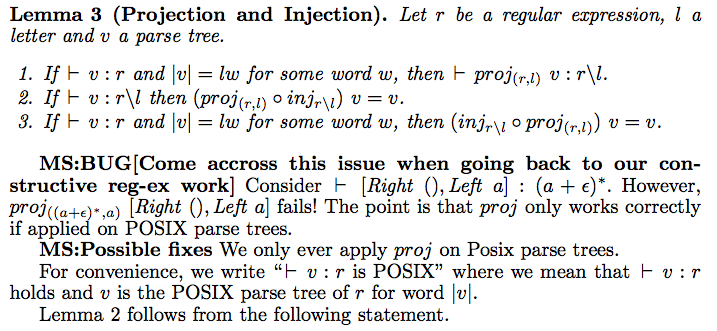
\includegraphics[scale=0.37]{pics/msbug.png}
  \end{bubble}
  \end{center}
  \end{textblock}}
  

\end{frame}
%%%%%%%%%%%%%%%%%%%%%%%%%%%%%%%%%%%%%%%%%%%%%%%%%%%%%%%%%%%%%%%%%% 

%%%%%%%%%%%%%%%%%%%%%%%%%%%%%%%%%%%%%%%%%%%%%%%%%%%%%%%%%%%%%%%%%%
\begin{frame}[c]
\frametitle{\begin{tabular}{c}The Proof Idea\\[-1mm] by Sulzmann \& Lu
\end{tabular}}

\begin{itemize}
\item introduce an inductively defined ordering relation 
\bl{$v \succ_r v'$} which captures the idea of POSIX matching

\item the algorithm returns the maximum of all possible
 values that are possible for a regular expression.\pause
 \bigskip\small
 
\item the idea is from a paper by Cardelli \& Frisch about 
GREEDY matching (GREEDY $=$ preferring instant gratification to delayed
repletion):

\item e.g.~given \bl{$(a + (b + ab))^*$} and string \bl{$ab$}

\begin{center}
\begin{tabular}{ll}
GREEDY: & \bl{$[Left(a), Right(Left(b)]$}\\
POSIX:  & \bl{$[Right(Right(Seq(a, b))))]$}  
\end{tabular}
\end{center} 
\end{itemize}

\end{frame}
%%%%%%%%%%%%%%%%%%%%%%%%%%%%%%%%%%%%%%%%%%%%%%%%%%%%%%%%%%%%%%%%%%%%%%%%%%%%

%%%%%%%%%%%%%%%%%%%%%%%%%%%%%%%%%%%%%%%%%%%%%%%%%%%%%%%%%%%%%%%%%%
\begin{frame}[c]
\frametitle{}
\centering


\bl{\infer{\vdash Empty : \epsilon}{}}\hspace{15mm}
\bl{\infer{\vdash Char(c): c}{}}\bigskip

\bl{\infer{\vdash Seq(v_1, v_2) : r_1\cdot r_2}{\vdash v_1 : r_1 \quad \vdash v_2 : r_2}}
\bigskip

\bl{\infer{\vdash Left(v) : r_1 + r_2}{\vdash v : r_1}}\hspace{15mm}
\bl{\infer{\vdash Right(v): r_1 + r_2}{\vdash v : r_2}}\bigskip

\bl{\infer{\vdash [] : r^*}{}}\hspace{15mm}
\bl{\infer{\vdash [v_1,\ldots, v_n] : r^*}
          {\vdash v_1 : r \quad\ldots\quad \vdash v_n : r}}

\end{frame}
%%%%%%%%%%%%%%%%%%%%%%%%%%%%%%%%%%%%%%%%%%%%%%%%%%%%%%%%%%%%%%%%%% 

%%%%%%%%%%%%%%%%%%%%%%%%%%%%%%%%%%%%%%%%%%%%%%%%%%%%%%%%%%%%%%%%%%
\begin{frame}<1>[c]
\frametitle{}
\small

%\begin{tabular}{@{}lll@{}}
%\bl{$POSIX(v, r)$} & \bl{$\dn$} & \bl{$\vdash v : r$}\\ 
% & &   \bl{$\wedge \;\;(\forall v'.\;\; \vdash v' : r \,\wedge\, |v'| = |v| 
%     \Rightarrow v \succ_{\alert<2>{r}} v')$}
%\end{tabular}\bigskip\bigskip\bigskip


\centering

%\bl{\infer{Seq(v_1, v_2) \succ_{\alert<2>{r_1\cdot r_2}} Seq(v'_1, v'_2)}
%   {v_1 = v'_1 \quad v_2 \succ_{\alert<2>{r_2}} v'_2}}\hspace{3mm}
%\bl{\infer{Seq(v_1, v_2) \succ_{\alert<2>{r_1\cdot r_2}} Seq(v'_1, v'_2)}
%   {v_1 \not= v'_1 \quad v_1 \succ_{\alert<2>{r_1}} v'_1}}
%\bigskip

%\bl{\infer{Left(v) \succ_{\alert<2>{r_1 + r_2}} Left(v')}
%          {v \succ_{\alert<2>{r_1}} v'}}\hspace{15mm}
%\bl{\infer{Right(v) \succ_{\alert<2>{r_1 + r_2}} Right(v')}
%          {v \succ_{\alert<2>{r_2}} v'}}\bigskip\medskip

%\bl{\infer{Left(v) \succ_{\alert<2>{r_1 + r_2}} Right(v')}
%          {length |v|  \ge length |v'|}}\hspace{15mm}
%\bl{\infer{Right(v) \succ_{\alert<2>{r_1 + r_2}} Left(v')}
%          {length |v| >  length |v'|}}\bigskip

%\bl{$\big\ldots$}

\end{frame}
%%%%%%%%%%%%%%%%%%%%%%%%%%%%%%%%%%%%%%%%%%%%%%%%%%%%%%%%%%%%%%%%%% 


%%%%%%%%%%%%%%%%%%%%%%%%%%%%%%%%%%%%%%%%%%%%%%%%%%%%%%%%%%%%%%%%%%
\begin{frame}[c]
\frametitle{Problems}

\begin{itemize}
\item Sulzmann: \ldots Let's assume \bl{$v$} is not 
    a $POSIX$ value, then there must be another one
    \ldots contradiction.\bigskip\pause

\item Exists?

\begin{center}
\bl{$L(r) \not= \varnothing \;\Rightarrow\; \exists v.\;POSIX(v, r)$}
\end{center}\bigskip\bigskip\pause

\item in the sequence case 
\bl{$Seq(v_1, v_2)\succ_{r_1\cdot r_2} Seq(v_1', v_2')$}, 
the induction hypotheses require
\bl{$|v_1| = |v'_1|$} and \bl{$|v_2| = |v'_2|$}, 
but you only know

\begin{center}
\bl{$|v_1| \;@\; |v_2| = |v'_1| \;@\; |v'_2|$}
\end{center}\pause\small

\item although one begins with the assumption that the two 
values have the same flattening, this cannot be maintained 
as one descends into the induction (alternative, sequence)
\end{itemize}

\end{frame}
%%%%%%%%%%%%%%%%%%%%%%%%%%%%%%%%%%%%%%%%%%%%%%%%%%%%%%%%%%%%%%%%%% 

%%%%%%%%%%%%%%%%%%%%%%%%%%%%%%%%%%%%%%%%%%%%%%%%%%%%%%%%%%%%%%%%%%
\begin{frame}[c]
\frametitle{Our Solution}

\begin{itemize}
\item a direct definition of what a POSIX value is, using
the relation \bl{$s \in r \to v$} (specification):\medskip

\begin{center}
\bl{\infer{[] \in \epsilon \to Empty}{}}\hspace{15mm}
\bl{\infer{c \in c \to Char(c)}{}}\bigskip\medskip

\bl{\infer{s \in r_1 + r_2 \to Left(v)}
          {s \in r_1 \to v}}\hspace{10mm}
\bl{\infer{s \in r_1 + r_2 \to Right(v)}
          {s \in r_2 \to v & s \not\in L(r_1)}}\bigskip\medskip

\bl{\infer{s_1 @ s_2 \in r_1 \cdot r_2 \to Seq(v_1, v_2)}
          {\small\begin{array}{l}
           s_1 \in r_1 \to v_1 \\
           s_2 \in r_2 \to v_2 \\
           \neg(\exists s_3\,s_4.\; s_3 \not= []
           \wedge s_3 @ s_4 = s_2 \wedge
           s_1 @ s_3 \in L(r_1) \wedge
           s_4 \in L(r_2))
           \end{array}}}
           
\bl{\ldots}           
\end{center}
\end{itemize}

\end{frame}
%%%%%%%%%%%%%%%%%%%%%%%%%%%%%%%%%%%%%%%%%%%%%%%%%%%%%%%%%%%%%%%%%%

%%%%%%%%%%%%%%%%%%%%%%%%%%%%%%%%%%%%%%%%%%%%%%%%%%%%%%%%%%%%%%%%%%
\begin{frame}[c]
\frametitle{Properties}

It is almost trival to prove:

\begin{itemize}
\item Uniqueness
\begin{center}
If \bl{$s \in r \to v_1$} and \bl{$s \in r \to v_2$} then
\bl{$v_1 = v_2$}.
\end{center}\bigskip

\item Correctness
\begin{center}
\bl{$lexer(r, s) = v$} if and only if \bl{$s \in r \to v$}
\end{center}
\end{itemize}\bigskip\bigskip\pause


You can now start to implement optimisations and derive
correctness proofs for them. But we still do not know whether

\begin{center}
\bl{$s \in r \to v$} 
\end{center}

is a POSIX value according to Sulzmann \& Lu's definition
(biggest value for \bl{$s$} and \bl{$r$})
\end{frame}
%%%%%%%%%%%%%%%%%%%%%%%%%%%%%%%%%%%%%%%%%%%%%%%%%%%%%%%%%%%%%%%%%% 

%%%%%%%%%%%%%%%%%%%%%%%%%%%%%%%%%%%%%%%%%%%%%%%%%%%%%%%%%%%%%%%%%%
\begin{frame}[c]
\frametitle{Conclusion}

\begin{itemize}

\item we replaced the POSIX definition of Sulzmann \& Lu by a
      new definition (ours is inspired by work of Vansummeren,
      2006)\medskip
  
\item their proof contained small gaps (acknowledged) but had
      also fundamental flaws\medskip

\item now, its a nice exercise for theorem proving\medskip

\item some optimisations need to be applied to the algorithm
      in order to become fast enough\medskip

\item can be used for lexing, is a small beautiful functional
      program
 
\end{itemize}

\end{frame}
%%%%%%%%%%%%%%%%%%%%%%%%%%%%%%%%%%%%%%%%%%%%%%%%%%%%%%%%%%%%%%%%%% 


%%%%%%%%%%%%%%%%%%%%%%%%%%%%%%%%%%%%%%%%%%%%%%%%%%%%%%%%%%%%%%%%%%
  \begin{frame}[b]
  \frametitle{
  \begin{tabular}{c}
  \mbox{}\\[13mm]
  \alert{\LARGE Questions?}
  \end{tabular}}

  \end{frame}
%%%%%%%%%%%%%%%%%%%%%%%%%%%%%%%%%%%%%%%%%%%%%%%%%%%%%%%%%%%%%%%%%%     

\end{document}


%%% Local Variables:  
%%% mode: latex
%%% TeX-master: t
%%% End: 

